\section{Durchführung}
\label{sec:Durchführung}

Zunächst wird der Spalt so verschoben, dass an dem Photoelement das Interferenzmuster gut zu sehen ist.
Dabei sollte das Hauptmaximum möglichst mittig liegen.
Anschließend wird die Distanz $L$ zwischen Spalt und Photoelement bestimmt, wie in \autoref{fig:messapperatur} zu sehen ist.

Da der Detektor auch ohne einfallendes Laserlicht einen sogenannten Offsetstrom $I_\text{Dunkel}$ emittiert, muss dieser vor jeder Messung bestimmt werden und später von den einzelnen Messwerten subtrahiert werden.
Dazu wird die angezeigte Stromstärke ohne Laserlicht gemessen und notiert.

Zu Beginn der Messung wird das Photoelement mittig ausgerichtet, sodass es an dem Hauptmaximum steht.
Nun wird es in kleinen Schritten verschoben. Die Größe dieser wird so gewählt, dass zwischen den einzelnen Maxima mehrere Messungen liegen, um so die spätere Ausgleichsrechnung besser durchführen zu können.
Sind mehrere Maxima in eine Verschiebungsrichtung gemessen, so wird der gleiche Prozess in die andere Richtung wiederholt.

Analog dazu wird ein zweiter Spalt und ein Doppelspalt ausgemessen.


\begin{figure}
    \centering
    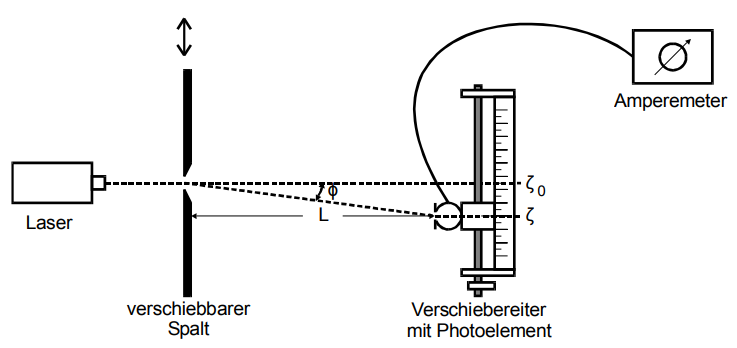
\includegraphics[width=0.9\textwidth]{content/messapperatur.png}
    \caption{Aufbau der Messapperatur zur Vermessung des Spaltes \cite{V406}.}
    \label{fig:messapperatur}
\end{figure}
